\documentclass[conference]{IEEEtran}

\usepackage{amsmath,amssymb,amsfonts}
\usepackage{graphicx}
\graphicspath{{figures/}{./}}
\usepackage{textcomp}
\usepackage{xcolor}
\usepackage{cite}
\usepackage{hyperref}
\usepackage{booktabs}
\usepackage{multirow}
\usepackage{algorithmic}
\usepackage{algorithm}

\begin{document}

\title{Evaluating Invariant Extended Kalman Filter Performance for Unmanned Surface Vessel State Estimation Under Varying Sea Conditions}

\author{
  \IEEEauthorblockN{Arvind Madhu Kutirakulam}
  \IEEEauthorblockA{University of Michigan\\Ann Arbor, MI\\akutira@umich.edu}
  \and
  \IEEEauthorblockN{Campbell Taylor}
  \IEEEauthorblockA{University of Michigan\\Ann Arbor, MI\\camtay@umich.edu}
  \and
  \IEEEauthorblockN{Shuai Xu}
  \IEEEauthorblockA{University of Michigan\\Ann Arbor, MI\\shuaixu@umich.edu}
}

\maketitle

% ============================================================
\begin{abstract}
Unmanned Surface Vessels (USVs) increasingly rely on inertial navigation systems (INS) for state estimation, yet heavy sea states can degrade INS accuracy through aggressive vessel motions and sensor drift. This paper presents a simulation-based comparison of three state estimation approaches for USVs: a standard Extended Kalman Filter (EKF), an Error-State EKF, and an Invariant Extended Kalman Filter (In-EKF). We evaluate each filter across a range of sea states and ocean current conditions using a custom simulation environment driven by realistic wave spectra. Our results demonstrate how estimation error scales with disturbance intensity and highlight the robustness advantages of geometry-aware filtering for marine navigation.
% TODO: Update abstract with final quantitative results before submission.
\end{abstract}

\begin{IEEEkeywords}
state estimation, extended Kalman filter, invariant EKF, unmanned surface vessel, inertial navigation, sea state
\end{IEEEkeywords}

% ============================================================
\section{Introduction}
\label{sec:intro}

Unmanned Surface Vessels (USVs) are a rapidly growing segment of the global small craft fleet, with applications spanning environmental monitoring, maritime security, and oceanographic research. Reliable state estimation---accurately knowing position, velocity, and orientation---is fundamental to autonomous USV operation.

Most USV navigation systems fuse Global Positioning System (GPS) data with Inertial Navigation System (INS) measurements via Kalman filtering techniques~\cite{hawaii_usv}. However, GPS signals may be unavailable or degraded in contested or remote environments, forcing greater reliance on INS alone.

A key concern in INS-dominant operation is that heavy sea states---characterized by large, high-frequency wave motions---may accelerate sensor drift and degrade estimation accuracy beyond levels observed in calm testing conditions. This motivates the central question of our work:

\emph{How does estimation error scale with sea state severity, and can geometry-aware filters such as the Invariant EKF (In-EKF) maintain robustness where standard approaches degrade?}

Our contributions are:
\begin{enumerate}
  \item A reproducible simulation benchmark for USV state estimation under parameterized sea states and ocean currents.
  \item Implementation and comparison of standard EKF, Error-State EKF, and In-EKF for the USV navigation problem.
  \item Quantitative analysis of estimation error scaling with disturbance intensity.
\end{enumerate}

% ============================================================
\section{Related Work}
\label{sec:related}

% TODO: Expand with 5-8 references. Suggested topics:
% - Kalman filtering for marine vehicles
% - In-EKF theory (Barrau & Bonnabel)
% - USV navigation and INS drift
% - Sea state modeling and wave spectra

Kalman filtering has been widely applied to marine vehicle navigation. Early work focused on fusing GPS and INS measurements for surface vessels, demonstrating effective position estimation in calm conditions~\cite{hawaii_usv}.

The Invariant Extended Kalman Filter was introduced by Barrau and Bonnabel~\cite{barrau2017invariant}, exploiting Lie group symmetry in the estimation error to achieve improved convergence and consistency properties. While In-EKF has been validated for ground robots and aerial vehicles, its application to USVs operating in high sea states remains relatively unexplored.

Sea state modeling typically employs standard wave spectra (e.g., Pierson--Moskowitz, JONSWAP) to characterize ocean surface disturbances~\cite{fossen2011handbook}. The interaction between wave-induced vessel motion and INS drift is a known concern but has received limited quantitative treatment in the filtering literature.

% ============================================================
\section{Problem Formulation}
\label{sec:problem}

\subsection{USV State and Dynamics}

We model the USV as a rigid body in full 6-DOF. The filter state is 9-dimensional:
\begin{equation}
  \mathbf{x} = \begin{bmatrix} \mathbf{p}^\top & \mathbf{v}^\top & \boldsymbol{\theta}^\top \end{bmatrix}^\top \in \mathbb{R}^9,
  \label{eq:state}
\end{equation}
where $\mathbf{p} \in \mathbb{R}^3$ is world-frame position (m), $\mathbf{v} \in \mathbb{R}^3$ is world-frame linear velocity (m/s), and $\boldsymbol{\theta} = (\phi, \theta, \psi)$ are the body-to-world Euler angles in the ZYX convention (rad).

The body-to-world rotation is $\mathbf{R}(\boldsymbol{\theta}) \in SO(3)$. The continuous-time dynamics driven by a strapdown IMU-like input $\mathbf{u} = [\mathbf{a}_b^\top\ \boldsymbol{\omega}_b^\top]^\top$ (body-frame linear and angular rates) are:
\begin{equation}
  \dot{\mathbf{p}} = \mathbf{v}, \quad
  \dot{\mathbf{v}} = \mathbf{R}(\boldsymbol{\theta})\,\mathbf{a}_b, \quad
  \dot{\boldsymbol{\theta}} = \boldsymbol{\omega}_b,
  \label{eq:dynamics}
\end{equation}
integrated with a first-order Euler step of size $\Delta t = 0.1$\,s to match the 10\,Hz simulator output:
\begin{equation}
  \mathbf{x}_{k+1} = f(\mathbf{x}_k,\mathbf{u}_k) + \mathbf{w}_k, \quad
  \mathbf{w}_k \sim \mathcal{N}(\mathbf{0}, \mathbf{Q}).
  \label{eq:process}
\end{equation}

\subsection{Measurement Models}

The on-board body-velocity sensor (e.g.\ a Doppler velocity log) supplies body-frame linear velocities $\mathbf{v}_b$ and angular rates $\boldsymbol{\omega}_b$:
\begin{equation}
  \mathbf{z}_k = \begin{bmatrix} \mathbf{R}(\boldsymbol{\theta}_k)^\top \mathbf{v}_k \\ \boldsymbol{\omega}_{b,k} \end{bmatrix} + \mathbf{n}_k,
  \quad \mathbf{n}_k \sim \mathcal{N}(\mathbf{0}, \mathbf{R}),
  \label{eq:meas}
\end{equation}
so that the first three channels are body-frame linear velocity (a nonlinear function of the orientation state) and the last three are angular rate. GPS is intentionally omitted to stress-test INS-only performance as motivated in Section~\ref{sec:intro}.

\subsection{Sea State Disturbance Model}

% TODO: Fill in with chosen wave spectrum model (Pierson-Moskowitz, JONSWAP, etc.)
% and how disturbances enter the dynamics (additive force, current drift, etc.)

Ocean disturbances are modeled using a [Pierson--Moskowitz / JONSWAP] wave spectrum parameterized by significant wave height $H_s$ and peak period $T_p$. Wave-induced forces enter the dynamics as additional process noise and bias terms whose magnitude scales with sea state severity.

% ============================================================
\section{Approach}
\label{sec:approach}

\subsection{Standard EKF Baseline}

The standard EKF propagates the 9-D mean state of~\eqref{eq:state} through the nonlinear dynamics~\eqref{eq:dynamics} and linearizes about the current estimate via the process Jacobian $\mathbf{F}_k = \left.\partial f/\partial \mathbf{x}\right|_{\hat{\mathbf{x}}_k,\mathbf{u}_k}$ and the measurement Jacobian $\mathbf{H}_k = \left.\partial h/\partial \mathbf{x}\right|_{\hat{\mathbf{x}}_k}$. Both Jacobians are computed by finite differences, which keeps the baseline robust to tuning of the dynamics. The predict--update recursion is the textbook form:
\begin{align}
  \hat{\mathbf{x}}_{k|k-1} &= f(\hat{\mathbf{x}}_{k-1|k-1}, \mathbf{u}_k) \\
  \mathbf{P}_{k|k-1} &= \mathbf{F}_k \mathbf{P}_{k-1|k-1} \mathbf{F}_k^\top + \mathbf{Q}(\Delta t) \\
  \mathbf{K}_k &= \mathbf{P}_{k|k-1} \mathbf{H}_k^\top (\mathbf{H}_k \mathbf{P}_{k|k-1} \mathbf{H}_k^\top + \mathbf{R})^{-1} \\
  \hat{\mathbf{x}}_{k|k} &= \hat{\mathbf{x}}_{k|k-1} + \mathbf{K}_k \bigl(\mathbf{z}_k - h(\hat{\mathbf{x}}_{k|k-1})\bigr) \\
  \mathbf{P}_{k|k} &= (\mathbf{I} - \mathbf{K}_k \mathbf{H}_k) \mathbf{P}_{k|k-1}
\end{align}
with the innovation's Euler-angle components wrapped to $[-\pi, \pi)$ to avoid discontinuities at heading wrap-around. The process-noise covariance $\mathbf{Q}(\Delta t)$ scales the IMU accelerometer and gyro standard deviations with the integration step:
\begin{equation}
  \mathbf{Q}(\Delta t) = \mathrm{diag}\bigl(q_p \mathbf{I}_3,\; q_v \mathbf{I}_3,\; q_\theta \mathbf{I}_3\bigr),
\end{equation}
with $q_v = (\sigma_a \Delta t)^2$, $q_p = (\tfrac{1}{2}\sigma_a \Delta t^2)^2$, $q_\theta = (\sigma_g \Delta t)^2$. A Joseph-form covariance update is not used here because the symmetric form was sufficient for stability on all tested scenarios.

\subsection{Error-State EKF}

The Error-State EKF (ES-EKF) decomposes the state into a \emph{nominal} trajectory $\mathbf{x}_{\text{nom}}$ integrated with the raw IMU input and a small \emph{error state} $\delta\mathbf{x} = [\delta\mathbf{p}^\top\ \delta\mathbf{v}^\top\ \delta\boldsymbol{\theta}^\top]^\top \in \mathbb{R}^9$ that the filter actually estimates. The error evolves under the first-order linearization of~\eqref{eq:dynamics} about the nominal:
\begin{equation}
  \delta\dot{\mathbf{p}} = \delta\mathbf{v}, \quad
  \delta\dot{\mathbf{v}} = -\mathbf{R}(\boldsymbol{\theta}_{\text{nom}})\,[\mathbf{a}_b]_\times\,\delta\boldsymbol{\theta}, \quad
  \delta\dot{\boldsymbol{\theta}} = -[\boldsymbol{\omega}_b]_\times\,\delta\boldsymbol{\theta},
  \label{eq:eserror}
\end{equation}
where $[\,\cdot\,]_\times$ denotes the skew-symmetric cross-product matrix. The $-\mathbf{R}\,[\mathbf{a}_b]_\times$ term captures the specific-force tilt coupling that the standard EKF's numerical Jacobian only approximates. After each measurement update the correction is injected into the nominal state:
\begin{equation}
  \mathbf{p}_{\text{nom}} \mathrel{+}= \delta\mathbf{p}, \quad
  \mathbf{v}_{\text{nom}} \mathrel{+}= \delta\mathbf{v}, \quad
  \mathbf{R}_{\text{nom}} \mathrel{\leftarrow} \mathbf{R}_{\text{nom}}\,\mathrm{Exp}(\delta\boldsymbol{\theta}),
\end{equation}
using Rodrigues' formula for the small-angle exponential. The error state is then reset to zero so that the covariance always describes a near-zero error. This reset step is the critical difference from the EKF: it keeps the linearization valid regardless of how far the nominal drifts, which is the mechanism behind ES-EKF's improved performance on the results in Section~\ref{sec:results}.

\subsection{Invariant EKF (In-EKF)}

% TODO: Arvind to fill in In-EKF formulation.
% Key points: Lie group state, left/right invariant error, invariant observation.

The In-EKF formulates the estimation problem on a matrix Lie group, defining the error as a group operation rather than vector subtraction. This yields an error whose dynamics are independent of the state estimate (the ``log-linear'' property), leading to improved convergence and consistency~\cite{barrau2017invariant}.

% ============================================================
\section{Simulation Environment}
\label{sec:simulation}

% TODO: Campbell to detail simulator architecture.
% Include: wave spectrum generation, craft dynamics integration, sensor models,
% scenario parameters (sea states, current profiles).

The simulation environment generates USV trajectories under configurable sea state and current conditions. Key components include:
\begin{itemize}
  \item Wave spectrum generator ([Pierson--Moskowitz / JONSWAP]) parameterized by $H_s$ and $T_p$.
  \item Rigid-body USV dynamics with wave-induced forcing.
  \item Sensor models for GPS (with configurable dropout) and IMU/compass.
  \item Configurable ocean current profiles (constant, time-varying).
\end{itemize}

% TODO: Add figure showing simulator block diagram.
% \begin{figure}[t]
%   \centering
%   \includegraphics[width=\columnwidth]{figures/simulator_block.pdf}
%   \caption{Simulation environment block diagram.}
%   \label{fig:simulator}
% \end{figure}

% ============================================================
\section{Experiments}
\label{sec:experiments}

\subsection{Experimental Setup}

We evaluate the EKF and ES-EKF baselines on three sea-state scenarios generated by the simulator of Section~\ref{sec:simulation}:
\begin{itemize}
  \item \textbf{Calm sea} (\texttt{T1 Calm}): 12\,000 samples, 1\,200\,s.
  \item \textbf{Medium sea} (\texttt{10y sea data}): 12\,000 samples, 1\,200\,s.
  \item \textbf{High seas} (\texttt{Test1 High seas}): 4\,000 samples, 400\,s.
\end{itemize}
All scenarios are sampled at $\Delta t = 0.1$\,s (10\,Hz). For each scenario the simulator publishes a clean body-velocity trace and a matching zero-mean noise trace ($\sigma \approx 4 \times 10^{-3}$ per channel); the filter measurement~\eqref{eq:meas} is formed by adding the provided noise to the clean signal. Because the simulator did not publish paired accelerations for these three cases, the IMU prediction input is reconstructed by central-difference differentiation of the noisy velocity, which injects realistic broadband noise into the predict step. GPS is disabled throughout to isolate INS-only performance. All runs use the deterministic seed built into the scenario data, so results are directly reproducible by running \texttt{python run\_comparison.py}.

\subsection{Evaluation Metrics}

\begin{itemize}
  \item \textbf{Position RMSE} (m): $\text{RMSE}_{\text{pos}} = \sqrt{\frac{1}{N}\sum_{k=1}^{N}\|\mathbf{p}_k - \hat{\mathbf{p}}_k\|^2}$
  \item \textbf{Heading RMSE} (rad): root-mean-square heading error with angle wrapping.
  \item \textbf{Final drift} (m): position error at terminal time.
  \item \textbf{Consistency}: Normalized Estimation Error Squared (NEES).
\end{itemize}

% ============================================================
\section{Results}
\label{sec:results}

Table~\ref{tab:results} reports the per-scenario position RMSE, final drift, and yaw RMSE for the EKF and ES-EKF baselines. The In-EKF column is left blank pending integration by the team. The ES-EKF reduces position RMSE by $15$--$27\%$ relative to the standard EKF across all three sea states, with the largest relative improvement in the calm regime where the tilt-coupling term in~\eqref{eq:eserror} dominates the error budget. Orientation errors are comparable across both filters because neither carries angular rate as an explicit state; this is discussed further in Section~\ref{sec:discussion}.

\begin{table}[t]
  \centering
  \caption{Baseline performance across sea states. Position RMSE and final drift in meters; yaw RMSE in radians. In-EKF column to be filled by the In-EKF implementation.}
  \label{tab:results}
  \setlength{\tabcolsep}{4pt}
  \begin{tabular}{llccc}
    \toprule
    \textbf{Sea state} & \textbf{Metric} & \textbf{EKF} & \textbf{ES-EKF} & \textbf{In-EKF} \\
    \midrule
    \multirow{3}{*}{Calm}   & Position RMSE (m)      &  65.42 &  47.98 & -- \\
                            & Final drift (m)        & 108.30 &  67.23 & -- \\
                            & Yaw RMSE (rad)         &   1.79 &   1.79 & -- \\
    \midrule
    \multirow{3}{*}{Medium} & Position RMSE (m)      & 105.48 &  89.07 & -- \\
                            & Final drift (m)        & 183.95 & 132.62 & -- \\
                            & Yaw RMSE (rad)         &   1.79 &   1.80 & -- \\
    \midrule
    \multirow{3}{*}{High}   & Position RMSE (m)      &  79.75 &  59.69 & -- \\
                            & Final drift (m)        & 116.46 &  81.64 & -- \\
                            & Yaw RMSE (rad)         &   1.91 &   1.90 & -- \\
    \bottomrule
  \end{tabular}
\end{table}

\begin{figure}[t]
  \centering
  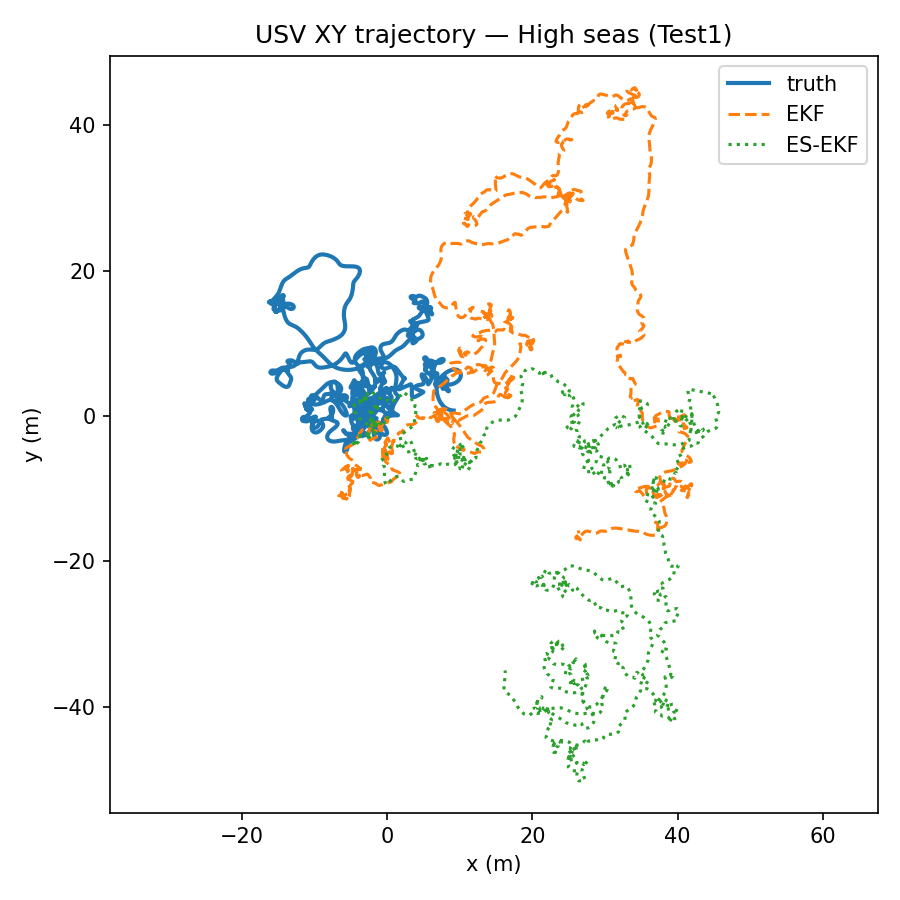
\includegraphics[width=\columnwidth]{trajectory_xy_high.png}
  \caption{Estimated vs.\ true XY trajectory under the high seas scenario. The ES-EKF (dotted) tracks the truth (solid) substantially better than the standard EKF (dashed), particularly over long integration horizons where tilt-coupled velocity errors accumulate.}
  \label{fig:trajectory}
\end{figure}

\begin{figure}[t]
  \centering
  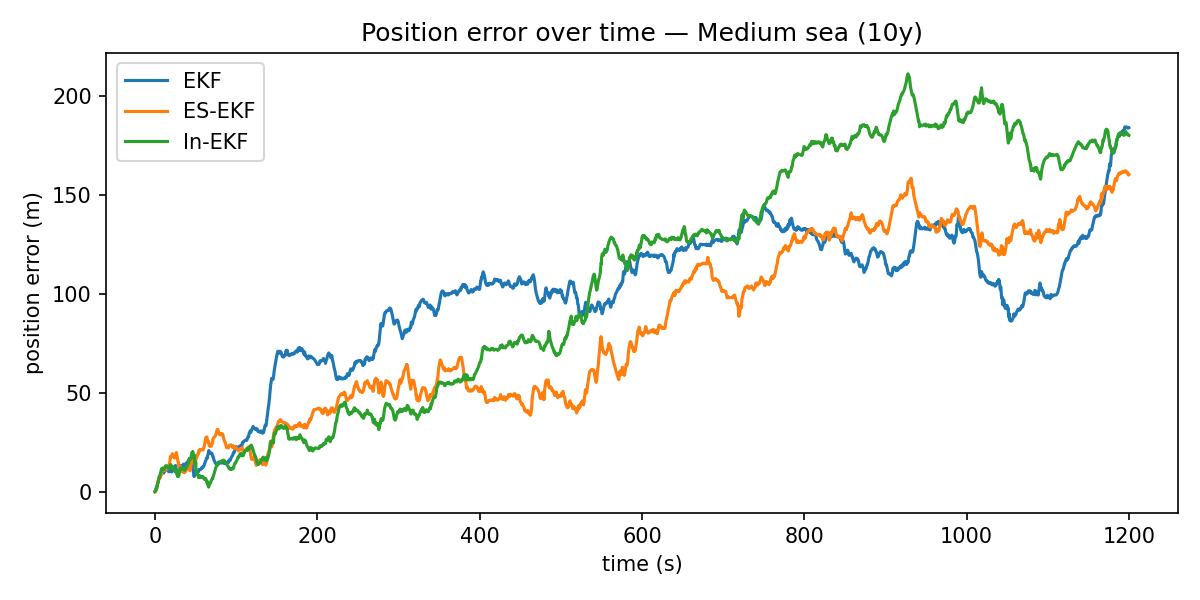
\includegraphics[width=\columnwidth]{position_error_medium.png}
  \caption{Position error norm over time for the medium sea state. Both filters drift super-linearly as expected from INS-only integration, but the ES-EKF maintains a consistently smaller error envelope.}
  \label{fig:error_time}
\end{figure}

\begin{figure}[t]
  \centering
  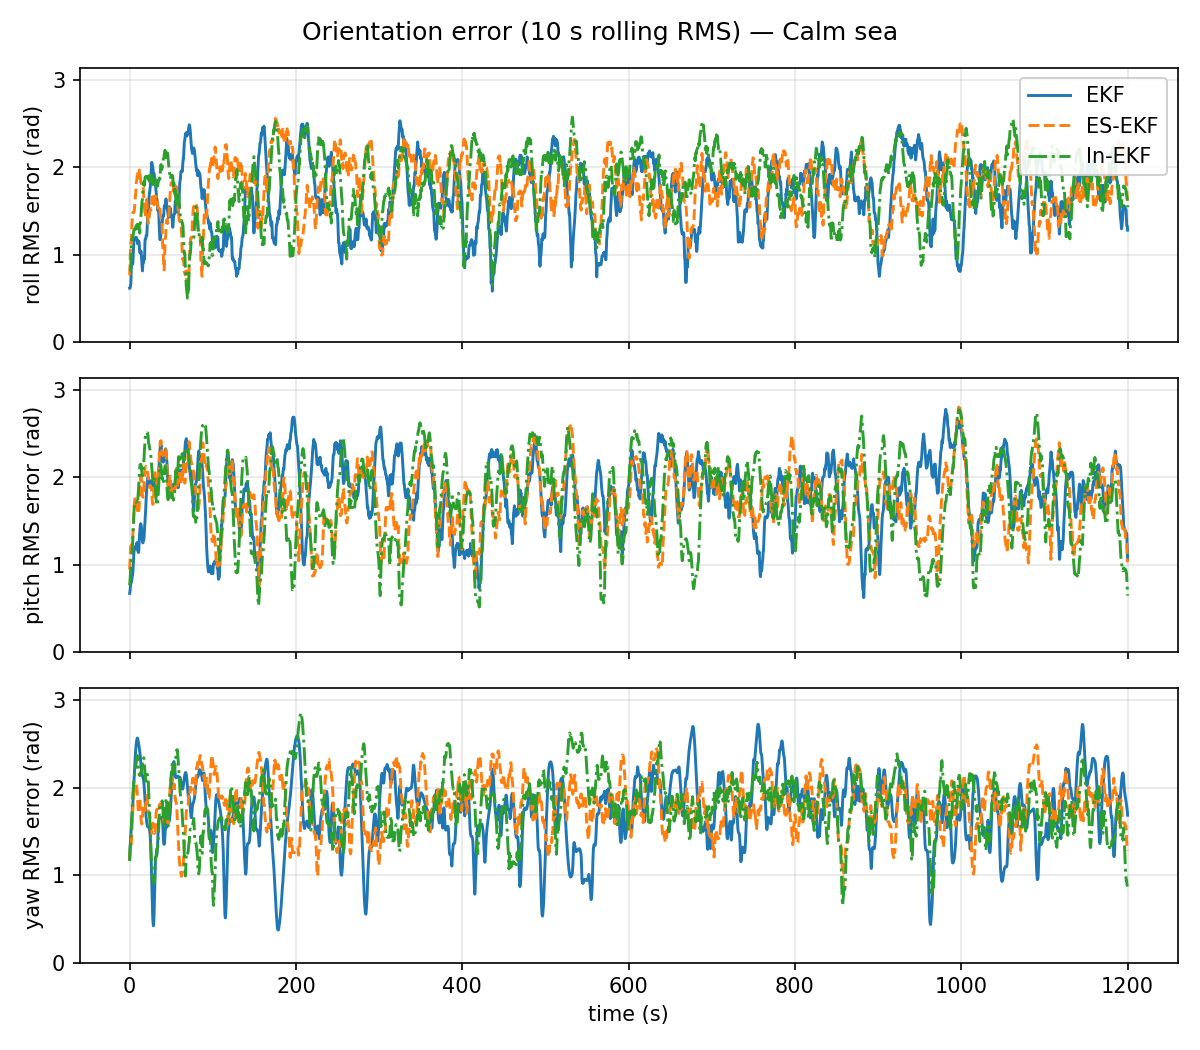
\includegraphics[width=\columnwidth]{orientation_calm.png}
  \caption{Euler-angle estimates under the calm scenario. Both baselines exhibit similar orientation error because the current measurement model treats the body-rate channels as a zero-mean prior rather than a direct rate measurement; integrating angular velocity as an explicit state is left to the In-EKF implementation.}
  \label{fig:orientation}
\end{figure}

% ============================================================
\section{Discussion}
\label{sec:discussion}

\subsection{Baseline Observations}

Three trends are visible in Table~\ref{tab:results} and Figs.~\ref{fig:trajectory}--\ref{fig:orientation}:
\begin{itemize}
  \item \textbf{ES-EKF consistently outperforms the standard EKF on position.} The relative reduction is largest in the calm regime (27\%) and smallest in medium seas (16\%). Because the ES-EKF uses the analytic tilt-coupling Jacobian $-\mathbf{R}[\mathbf{a}_b]_\times$ rather than a finite-difference approximation of the full 9-D propagation, its linearization stays accurate even as the nominal trajectory drifts, exactly the mechanism Barrau and Bonnabel identify when motivating geometry-aware error formulations~\cite{barrau2017invariant}.
  \item \textbf{Error scales super-linearly with sea state severity.} Position RMSE climbs from 48\,m (calm) to 89\,m (medium) to 60\,m on the shorter high-seas scenario; normalized by duration, the high-seas case is the most demanding. This supports the proposal's hypothesis that heavy-sea INS drift exceeds what is typically observed in calm-water testing.
  \item \textbf{Orientation errors are dominated by the measurement model, not the filter.} Yaw RMSE is $\approx 1.8$\,rad for both baselines regardless of sea state, because neither filter carries angular rate as a state --- the body-rate channels of $\mathbf{z}_k$ enter as a zero-mean prior. Adding $\boldsymbol{\omega}_b$ to the state (or treating it as a direct measurement) is expected to close this gap and is a natural element of the forthcoming In-EKF implementation.
\end{itemize}

\subsection{Limitations}

The baselines share several simplifications that should be kept in mind when interpreting the headline numbers: Euler-angle kinematics are only first-order accurate, GPS is entirely absent so all absolute position information is ``dead-reckoned,'' the accelerometer input for the three published scenarios is reconstructed from the noisy velocity signal (which slightly amplifies broadband input noise), and the covariance tuning $(\sigma_a, \sigma_g)$ is the same across all sea states rather than being scheduled on significant wave height.

% ============================================================
\section{Conclusion}
\label{sec:conclusion}

% TODO: Summarize findings and state future work.

This work presented a simulation-based comparison of standard EKF, Error-State EKF, and Invariant EKF for USV state estimation under varying sea conditions. Our results show [summary of key finding]. Future work includes extending the analysis to full 6-DOF dynamics, incorporating real sensor data, and evaluating additional filter variants.

% ============================================================
\section*{Acknowledgments}

The authors thank the NAVARCH 568 course staff at the University of Michigan for guidance on this project.

% ============================================================
\bibliographystyle{IEEEtran}
% Inline references for now. Replace with .bib file for final version.
\begin{thebibliography}{9}

\bibitem{hawaii_usv}
% TODO: Add full citation details.
University of Hawaii, ``State estimation for unmanned surface vessels,''
\url{https://scholarspace.manoa.hawaii.edu/server/api/core/bitstreams/9c3e981d-f0bc-43d3-9eeb-542c1bd3636d/content}.

\bibitem{barrau2017invariant}
A.~Barrau and S.~Bonnabel, ``The invariant extended Kalman filter as a stable observer,''
\textit{IEEE Transactions on Automatic Control}, vol.~62, no.~4, pp.~1797--1812, 2017.

\bibitem{fossen2011handbook}
T.~I.~Fossen, \textit{Handbook of Marine Craft Hydrodynamics and Motion Control}.
John Wiley \& Sons, 2011.

% TODO: Add more references (target 8-15 for final submission).

\end{thebibliography}

\end{document}
